\textbf{3-1} 如光图3-1-1所示，波长 $\lambda = 500\mathrm{nm}$ 的单色点光源 $S$ 与光阑的距离 $R_0 = 1\mathrm{m}$ ，光阑上有一个通光的圆环，内半径 $a_1 = 0.5\mathrm{mm}$ ，外半径 $a_2 = 1\mathrm{mm}$ ，光轴上 $P$ 点与光阑的距离 $r_0 = 1\mathrm{m}$ 。试求 $P$ 点的光强与没有光阑时 $P$ 点的光强之比。


\begin{center}
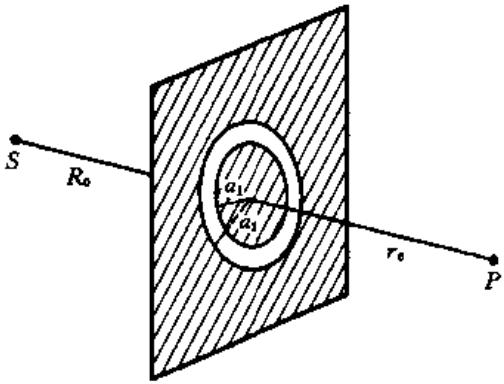
\includegraphics[width=0.2\textwidth]{figures/光图3-1-1.jpg}
\end{center}
\vfill

\textbf{3-2}如光图3-2-1所示，在菲涅耳圆孔衍射实验中，圆孔半径 $\rho = 2.0\mathrm{mm}$ ，点光源与圆孔的距离为 $R= 2.0 m$, 光波波长 $\lambda = 500$ nm. 当观察幕从很远处向圆孔移近时, 试求: 

1. 前三次出现中心亮斑(强度为极大)时幕的位置;

2. 前三次出现中心暗斑(强度为极小)时幕的位置. 

3. 当幕离圆孔的距离为 b = 5.0 m 时, 固定其位置, 逐渐扩大圆孔半径, 试求最先出现中心暗斑和亮斑时圆孔的半径.
\begin{center}
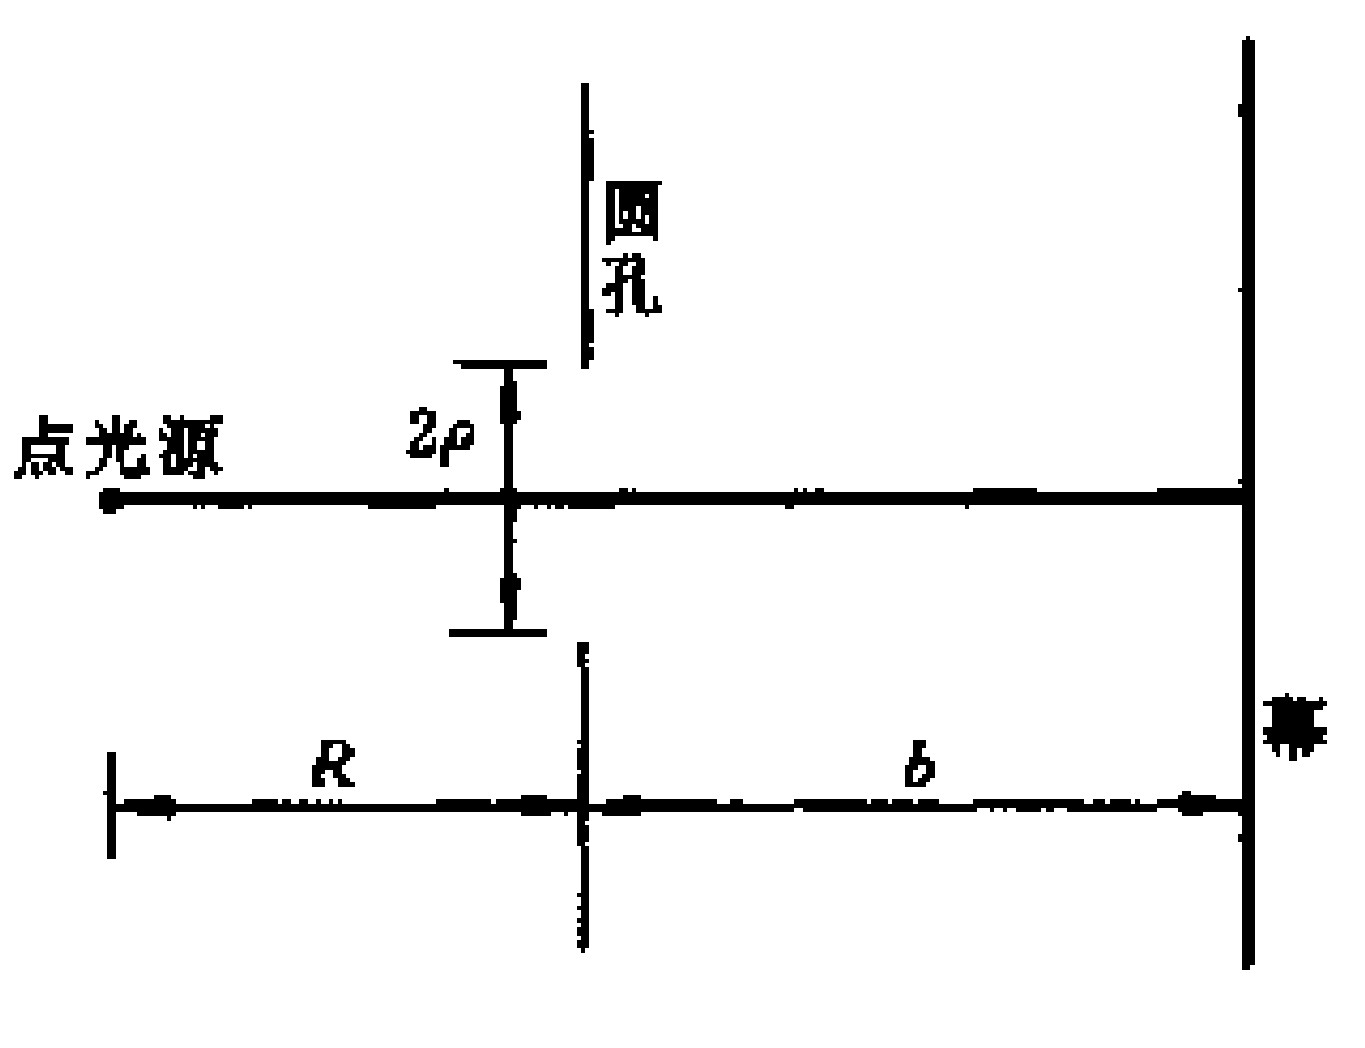
\includegraphics[width=0.2\textwidth]{figures/光图3-2-1.jpg}
\end{center}

\vfill
\newpage

\textbf{3-3} 波长 $\lambda = 550\mathrm{nm}$ 的平行单色光，光强为 $I_0$ ，垂直入射到直径 $d = 1.1\mathrm{mm}$ 的圆孔上，轴上一点 $P$ 与圆孔的距离 $r_0 = 33~\mathrm{cm}$ .

1.试求 $P$ 点的光强.

2.若在圆孔处放置一个焦距为 $33~\mathrm{cm}$ 的会聚薄透镜，试求 $P$ 点的光强.

\vfill
\newpage

\textbf{3-4} 一菲涅耳波带片包含偶数个波带，其中奇数波带是透明的，偶数波带不透明。第一个透明波带的直径 $d = 1\mathrm{mm}$ ，单色点光源波长 $\lambda = 500\mathrm{nm}$ 。

1. 已知轴上点光源位于波带片前方 $1\mathrm{m}$ 处。试求像点位置。

2. 若用相同孔径的透镜代替波带片，其焦距等于波带片的主焦距。试问其像点的光强是波带片主像点光强的多少倍？

\vfill
\textbf{3-5} 单缝缝宽为 $a$ ，波长为 $\lambda$ 的单色平行光垂直入射。缝宽的一半复盖一相对位型掩膜，使人射光经掩膜后相对狭缝的另一半产生 $\pi$ 的相移。

1. 试求夫琅禾费衍射的强度分布公式。

2. 设缝宽 $a = 10\lambda$ ，试画出强度分布曲线。

\vfill
\newpage
\textbf{3-6} 单缝缝宽为 $a$ ，复盖一振幅型掩膜．若以缝中心为原点，与缝垂直的方向取为 $x$ 轴．设经掩膜后的振幅透射率为
$$ t (x) = \cos \frac {\pi}{a} x $$
波长为 $\lambda$ 的单色平行光垂直入射。

1. 试求夫琅禾费衍射的强度分布公式, 并确定极小值的位置. 

2. 试求相邻两极小中点处的强度与中央极大强度之比.

\vfill
\textbf{3-7} 如光图3-7-1所示，两狭缝宽度不等，分别为 $a_1$ 和 $a_2$ ，双缝中心间距为 $d$ ，波长为 $\lambda$ 的单色平行光垂直入射.

1.试求夫琅禾费衍射的强度分布公式.

2.如光图3-7-1中，设 $a_1 = 2a_2 = 2a, d = 3a.$ 试讨论强度分布的特点.

\begin{center}
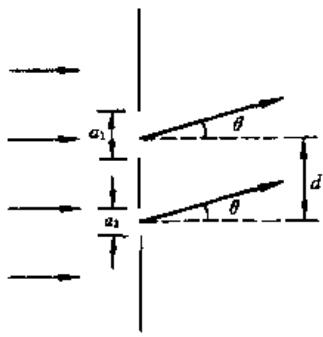
\includegraphics[width=0.3\textwidth]{figures/光图3-7-1.jpg}
\end{center}

\vfill
\newpage
\textbf{3-8} 如光图3-8-1所示，三平行狭缝的缝宽均为 $a$ ，相邻两缝的间距均为 $d$ ，中间狭缝前放置一透明相板, 它可使相位改变 $\pi$ , 波长为 $\lambda$ 的单色平行光正入射, 在透镜后焦面上观察衍射花样.

1. 试导出幕上的强度分布公式.

2. 试求一级衍射极小,一级干涉极大和一级干涉极小的位置.

\begin{center}
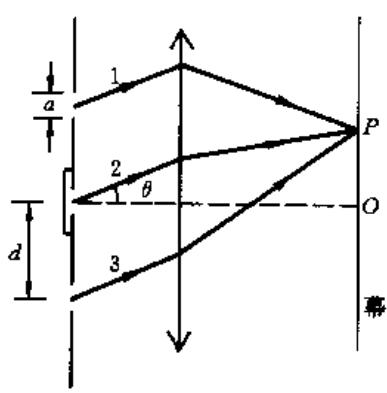
\includegraphics[width=0.4\textwidth]{figures/光图3-8-1.jpg}
\end{center}

\vfill
\newpage

\textbf{3-9} 如光图3-9-1所示，在夫琅禾费圆孔衍射实验中，单色平行光垂直入射到半径为 $a$ 的圆孔上。观察幕上任一点 $P$ 的强度为
$$ I (P) = I _ {0} \left[ \frac {2 J _ {1} (x)}{x} \right] ^ {2} $$
式中 $J_{1}$ 是一阶贝塞耳函数, 式中
$$ x = \frac {2 \pi}{\lambda} a \sin \theta $$
在小角衍射条件下，
$$ x = \frac {2 \pi a}{f \lambda} r $$
式中 f 为透镜焦距, r 是 P 点与衍射环环心 O 的距离, $I_{0}$ 为环心光强, $I_{0}$ 与入射光在圆孔面上的振幅 $A_{0}$ 以及圆孔面积 $\pi a^{2}$ 等有关, 具体表示式为
$$ I _ {0} = \frac {A _ {0} ^ {2} (\pi a ^ {2}) ^ {2}}{\lambda^ {2} f ^ {2}} $$
在幕上以 O 为中心，以 $r_{0}$ 为半径作一圆。试求落到该圆内的能量与入射到圆孔的总能量的比值，并进一步计算受里斑所占能量的百分数。
\begin{center}
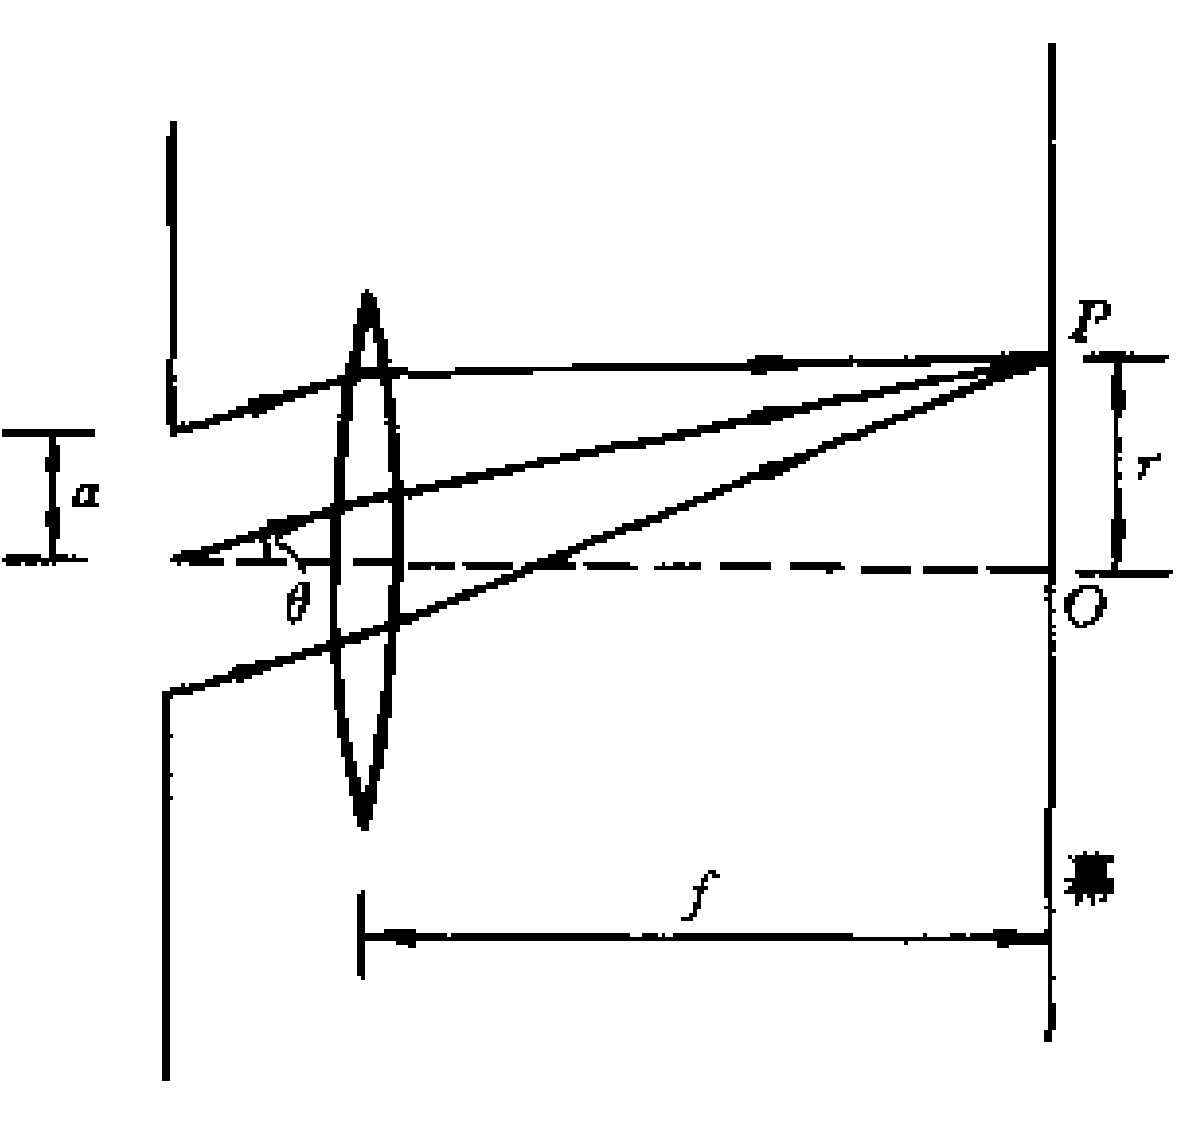
\includegraphics[width=0.4\textwidth]{figures/光图3-9-1.jpg}
\end{center}


\vfill
\newpage
\textbf{3-10} 如光图3-10-1所示，一通光圆环，其外半径为 $a$ ，内半径为 $b$ ，波长为 $\lambda$ 的单色平行光垂直入射.

1.试求夫琅禾费衍射强度分布公式.

2.若 $a = 2b$ ，试求环孔衍射和半径为 $a$ 的圆孔衍射的中央极大强度之比.

3.若 $a = 2b$ ，试求环孔衍射第一个暗环的角半径.

\begin{center}
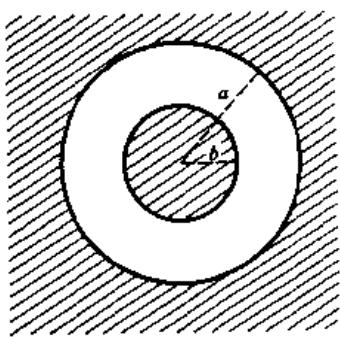
\includegraphics[width=0.2\textwidth]{figures/光图3-10-1.jpg}
\end{center}

\vfill
\textbf{3-11} 在夫琅禾费圆孔衍射实验中，在观察屏前表面放置一带孔遮板，如光图3-11-1所示，孔的形态有如下三种：

1. 衍射环中心的小圆孔，

2. 半径足够大的扇形，

3. 沿半径方向的等宽狭缝。

设衍射孔的半径为 $a$ ，试证明通过上述三孔的光通量依次正比于 $a^4, a^2$ 和 $a^3$ 。

\begin{center}
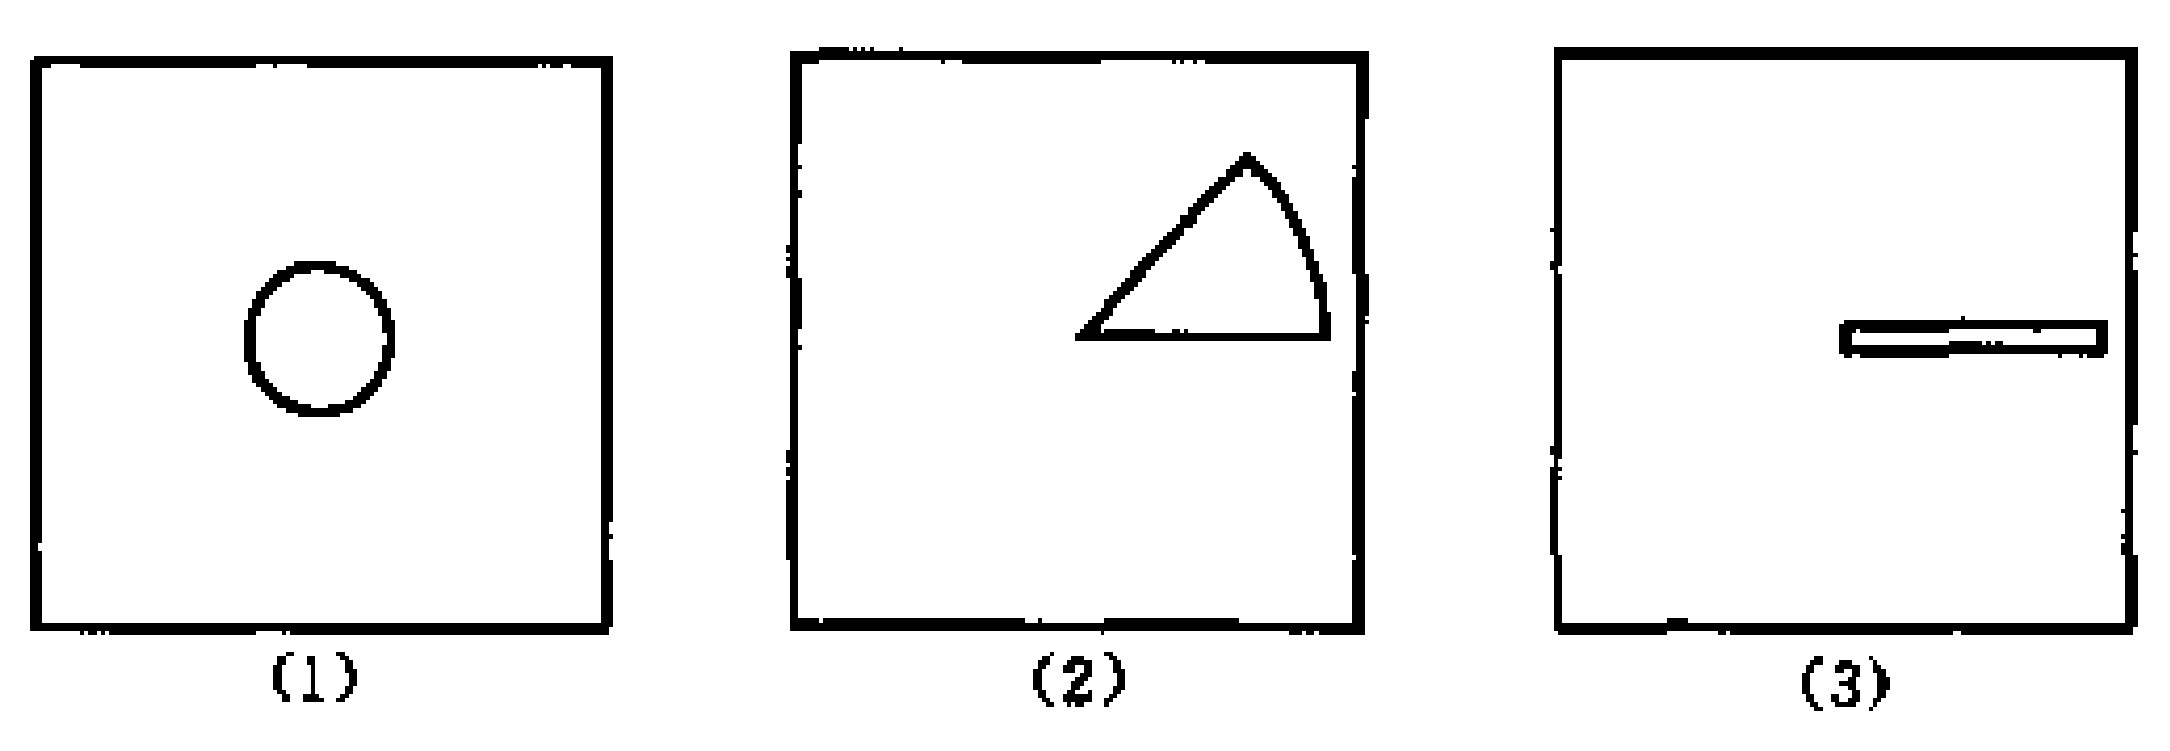
\includegraphics[width=0.5\textwidth]{figures/光图3-11-1.jpg}
\end{center}

\vfill
\newpage
\textbf{3-12} 试设计一透射光栅,要求:

1. 使波长 $\lambda = 600 \mathrm{~nm}$ 的第二级谱线的衍射角 $\theta \leqslant 30^{\circ}$ , 在此前提下角色散率要尽可能大.

2. 第三级光谱缺级.

3. 该波长的二级谱线附近至少能分辨 $0.02 \mathrm{~nm}$ 的波长差. 

满足上述要求的光栅的参数设定后, 试问能看到几级波长为 $600 \mathrm{~nm}$ 的谱线.

\vfill
\textbf{3-13} 试导出光栅干涉次极大位置的近似公式，并求最靠近主极大的次级大强度与主极大强度的比值。

\vfill
\newpage
\textbf{3-14} 一显微镜物镜的数值孔径N.A.=0.65,物与物镜之间为空气,对人眼最灵敏的黄绿光的波长为 $\lambda=550\ nm$ .

1. 试求显微镜的最小分辨距离.

2. 换用油浸物镜, 油的折射率 $n = 1.6$ , 仍用黄绿光, 试问最小分辨距离变为多少?

3. 仍用普通物镜, 但改用 $\lambda = 420 \mathrm{~nm}$ 的光, 试问最小分辨距离变为多少?4. 为充分利用第2问的分辨本领, 试问显微镜的放大倍数 (视角放大率) 应设计为多大? 设人眼瞳孔直径为 $2.5 \mathrm{~mm}$ .

\vfill
\textbf{3-15} 一光栅共有2N条缝宽均为a的狭缝，缝间不透明部分的宽度依次按 $a,3a,a,3a,\dots$ 周期性地变化，波长为 $\lambda$ 的单色光垂直入射。试求夫琅禾费衍射的强度分布。

\vfill
\newpage
\textbf{3-16} 一光栅的总缝数为 $2N$ ，光栅常量为 $d$ 。由于刻制过程的差错，第 $N$ 条缝和 $(N + 1)$ 条缝的间距不是 $d$ ，而是一任意值 $l$ 。试问此光栅与完善的光栅相比，干涉极大的性质有何异同。

\vfill
\textbf{3-17} 一衍射光栅每毫米有300条缝，入射光包含红光和紫光两种成分，垂直入射。发现在24.46°角度处的谱线同时含有红光和紫光两种成分。

1. 试问在什么角度处还会出现这种复合谱线。

2. 试问在什么角度处有单一的红光谱线出现。

\vfill
\newpage
\textbf{3-18} 如光图3-18-1所示，一闪耀光栅宽 $200\mathrm{mm}$ ，每毫米有500个刻槽，闪耀角 $\theta_B = 43^{\circ}26'$ ，平行光垂直于槽面入射。试求:

1. 对波长 $\lambda=550nm$ 的光的闪耀级次和色分辨本领.

2. 在闪耀方向的角色散率.3. 若入射光垂直光栅平面,则三级光谱中强度最大的波长是什么?

\begin{center}
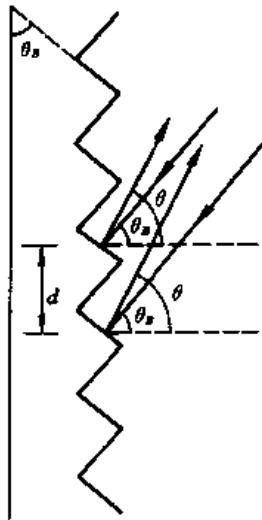
\includegraphics[width=0.13\textwidth]{figures/光图3-18-1.jpg}
\end{center}

\vfill
\textbf{3-19} 如光图3-19-1所示，透射式阶梯光栅由一系列厚度均为 $t$ ，折射率均为 $\pmb{n}$ 的玻璃板构成, 一板要比另一板伸出 $d$ 的距离. 平行光垂直入射, 用透镜接收衍射光, 在透镜后焦面上观察夫琅禾费衍射花样. 在衍射角 $\theta$ 很小的条件下, 

1. 试导出衍射强度分布公式, 并求干涉极大的角位置. 

2. 对 $n = 1.5, t = 0.5 \mathrm{~cm}, \lambda = 500 \mathrm{~nm}$ , 以及 40 阶的光栅, 试求 $\theta = 0$ 附近的干涉级次, 角色散率公式和色分辨本领. 

3. 综述阶梯光栅的特性.


\begin{center}
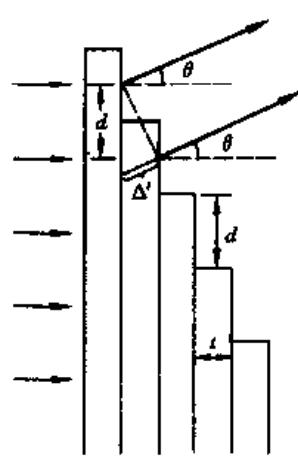
\includegraphics[width=0.2\textwidth]{figures/光图3-19-1.jpg}
\end{center}

\vfill
\newpage
\textbf{3-20} 设制作全息光栅时，两束相干平行光的传播方向与感光片法线所夹的角度分虽为 $\theta_{1}$ 和 $\theta_{2}$ ，光波波长为 $\lambda$ ，曝光后再经显影处理，假设乳胶特性是线性的。

1. 试求所得全息底片的振幅透射率。

2. 以上述全息光栅为衍射器件，并以原来的相干平行光垂直入射，试求夫琅禾费衍射的强度分布公式。

\vfill
\textbf{3-21} 制作上题(本章题20)的全息光栅时，设两束相干光的强度比为 $R = \left(\frac{A}{B}\right)^2$ 。1. 试求入射到感光片的光强分布的反衬度。2. 试证明全息光栅的衍射效率与反衬度的平方成反比。3. 试定性讨论束强比 $R$ 的取值原则。

\vfill
\newpage
\textbf{3-22} 如光图3-22-1所示，全息感光片放置在 $z = 0$ 的 $xy$ 平面上，平行的参考光沿 $xz$ 平面入射，其波矢 $\pmb{k}$ 与 $z$ 轴夹 $\theta$ 角，物点坐标为 $(x_0, y_0 - d_0)$ ， $d_0$ 是物点到感光片的垂直距离。感光片同时接收参考光和从物点发出的球面波，经显影处理后制成全息片。以原参考光照明全息片。

试证明在全息片后的±1级衍射光分别形成物点的虚像和实像，并求两像点的位置。

\begin{center}
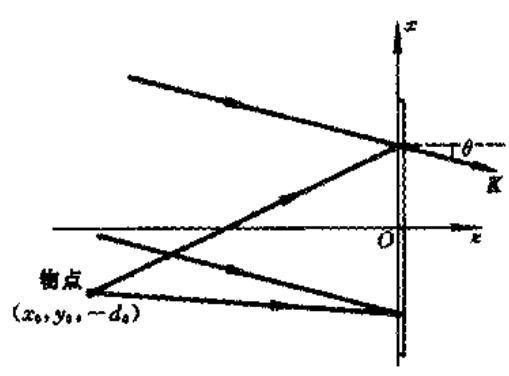
\includegraphics[width=0.3\textwidth]{figures/光图3-22-1.jpg}
\end{center}

\vfill
